% =====================================================================
%  Diagrama 6 — Proceso de gestión de riesgos en los requisitos
%  Adapta la figura 9.1 del capítulo 9 de referencia al caso RedPepper:
%  el ciclo identificar -> analizar -> evaluar -> tratar se repite en cada
%  etapa (educción, ilación y especificación), dentro de un marco de
%  registro, control y retroalimentación.
%  Se incluye desde diagramas/fuentes/ y se exporta a PNG de 300 dpi.
% =====================================================================
% =====================================================================
%  estilo.tex — sistema visual común de los diagramas RedPepper
%  Se incluye desde cada figura (documento independiente).
% =====================================================================
\documentclass[11pt,tikz,border=6pt]{standalone}

\usepackage[utf8]{inputenc}
\usepackage[T1]{fontenc}
\usepackage{lmodern}
\usepackage{helvet}
\renewcommand{\familydefault}{\sfdefault}

\usepackage{tikz}
\usetikzlibrary{positioning,arrows.meta,shapes.geometric,fit,backgrounds,calc}

% --- Paleta por rol (tonos suaves, legibles en impresión) ---------------
\definecolor{cCliente}{HTML}{FFF1D6}
\definecolor{bCliente}{HTML}{B8860B}
\definecolor{cCaja}{HTML}{E4F2E1}
\definecolor{bCaja}{HTML}{3E7D3A}
\definecolor{cSistema}{HTML}{E3ECF9}
\definecolor{bSistema}{HTML}{2F5D9E}
\definecolor{cCocina}{HTML}{FBE5E3}
\definecolor{bCocina}{HTML}{A33B33}
\definecolor{cAdmin}{HTML}{EDEDED}
\definecolor{bAdmin}{HTML}{555555}
\definecolor{cProveedor}{HTML}{F0E7F7}
\definecolor{bProveedor}{HTML}{6A4C93}
\definecolor{cContador}{HTML}{DEF1EF}
\definecolor{bContador}{HTML}{2E7D74}

% --- Estilos ------------------------------------------------------------
\tikzset{
  proc/.style={
    draw=black!55, rounded corners=3pt, fill=white, align=center,
    font=\small,
    execute at begin node={\hyphenpenalty=10000\exhyphenpenalty=10000},
    inner sep=3.5pt, minimum height=0.95cm, text width=3.05cm
  },
  cliente/.style={proc, fill=cCliente, draw=bCliente},
  caja/.style={proc, fill=cCaja, draw=bCaja},
  sistema/.style={proc, fill=cSistema, draw=bSistema},
  cocina/.style={proc, fill=cCocina, draw=bCocina},
  admin/.style={proc, fill=cAdmin, draw=bAdmin},
  proveedor/.style={proc, fill=cProveedor, draw=bProveedor},
  contador/.style={proc, fill=cContador, draw=bContador},
  dec/.style={
    diamond, aspect=2.1, draw=black!60, fill=white, align=center,
    font=\footnotesize, inner sep=1pt, minimum width=2.6cm, minimum height=1.15cm
  },
  ini/.style={
    draw=black!60, rounded corners=14pt, fill=black!6, align=center,
    font=\footnotesize\bfseries, inner sep=5pt, minimum height=0.9cm, text width=2.6cm
  },
  flecha/.style={-{Stealth[length=2.2mm,width=1.6mm]}, draw=black!70, line width=0.7pt},
  flechad/.style={flecha, dashed},
  etiqueta/.style={font=\scriptsize, inner sep=2pt, fill=white, draw=none, text=black!75},
  banda/.style={fill=black!82, text=white, font=\small\bfseries, align=center, inner sep=4pt},
  leyenda/.style={font=\scriptsize, align=left, text=black!80}
}

% --- Encabezado y leyenda ----------------------------------------------
% #1 ancho total, #2 título, #3 y del encabezado
\newcommand{\encabezado}[3]{%
  \node[banda, minimum width=#1, minimum height=0.62cm, anchor=north west]
    at (-0.45,#3) {\strut #2};%
}
% #1 x, #2 y  (leyenda en dos filas para evitar solapamientos)
\newcommand{\leyendaRoles}[2]{%
  \begin{scope}[shift={(#1,#2)}]
    \foreach \x/\c/\b/\t in {0/cCliente/bCliente/Cliente,
                              2.7/cCaja/bCaja/Caja,
                              5.2/cSistema/bSistema/Sistema,
                              8.4/cCocina/bCocina/Cocina}{%
      \node[draw=\b, fill=\c, minimum width=0.34cm, minimum height=0.24cm,
            anchor=west] at (\x,0) {};
      \node[leyenda, anchor=west] at ({\x+0.24},0) {\t};%
    }
    \foreach \x/\c/\b/\t in {0/cAdmin/bAdmin/Administración,
                              3.4/cProveedor/bProveedor/Proveedor,
                              6.6/cContador/bContador/Contador}{%
      \node[draw=\b, fill=\c, minimum width=0.34cm, minimum height=0.24cm,
            anchor=west] at (\x,-0.42) {};
      \node[leyenda, anchor=west] at ({\x+0.24},-0.42) {\t};%
    }
  \end{scope}
}


\definecolor{cLoop}{HTML}{B45309}

\begin{document}
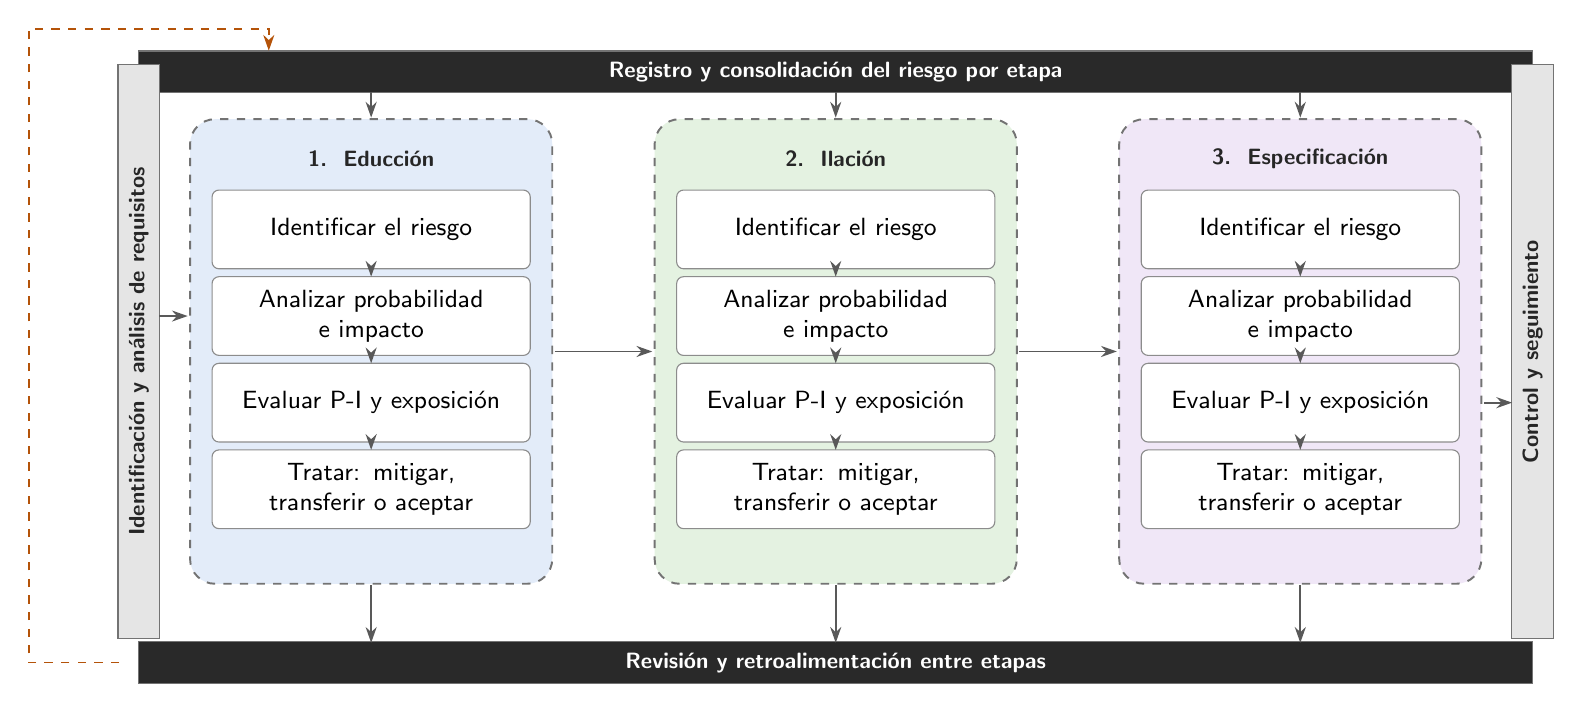
\begin{tikzpicture}[
  etapa/.style={rounded corners=9pt, draw=black!55, dashed, line width=0.7pt,
                fill=#1, inner sep=6pt},
  paso/.style={draw=black!45, rounded corners=2.5pt, fill=white,
               font=\small, align=center, minimum height=1.0cm,
               text width=3.9cm, inner sep=2pt,
               execute at begin node={\hyphenpenalty=10000\exhyphenpenalty=10000}},
  banda/.style={draw=black!55, fill=black!84, text=white,
                font=\footnotesize\bfseries, align=center, inner sep=4pt,
                minimum height=0.5cm},
  rail/.style={draw=black!55, fill=black!10, text=black!85,
               font=\footnotesize\bfseries, align=center, inner sep=4pt},
  flujo/.style={-{Stealth[length=2mm,width=1.4mm]}, draw=black!65,
                line width=0.7pt},
  flujod/.style={flujo, dashed},
  nota/.style={font=\footnotesize, align=center, text=black!70}
]

  \def\dxA{0}
  \def\dxB{5.9}
  \def\dxC{11.8}
  \def\yTop{3.55}
  \def\yBot{-3.95}

  % ---------------- Etapas ----------------
  \node[etapa=cSistema,   minimum width=4.6cm, minimum height=5.9cm] (cA) at (\dxA,0) {};
  \node[etapa=cCaja,      minimum width=4.6cm, minimum height=5.9cm] (cB) at (\dxB,0) {};
  \node[etapa=cProveedor, minimum width=4.6cm, minimum height=5.9cm] (cC) at (\dxC,0) {};

  \node[font=\footnotesize\bfseries, text=black!85] at (\dxA,2.45) {1.\ \ Educción};
  \node[font=\footnotesize\bfseries, text=black!85] at (\dxB,2.45) {2.\ \ Ilación};
  \node[font=\footnotesize\bfseries, text=black!85] at (\dxC,2.45) {3.\ \ Especificación};

  \foreach \dx in {\dxA,\dxB,\dxC}{
    \node[paso] at (\dx,1.55) {Identificar el riesgo};
    \node[paso] at (\dx,0.45) {Analizar probabilidad e impacto};
    \node[paso] at (\dx,-0.65) {Evaluar P-I y exposición};
    \node[paso] at (\dx,-1.75) {Tratar: mitigar, transferir o aceptar};
    \draw[flujo] (\dx,1.05) -- (\dx,0.95);
    \draw[flujo] (\dx,-0.05) -- (\dx,-0.15);
    \draw[flujo] (\dx,-1.15) -- (\dx,-1.25);
  }

  % ---------------- Marco: bandas superior e inferior ----------------
  \node[banda, minimum width=17.7cm] at (\dxB,\yTop) {Registro y consolidación del riesgo por etapa};
  \node[banda, minimum width=17.7cm] at (\dxB,\yBot) {Revisión y retroalimentación entre etapas};

  \node[rail, rotate=90, minimum width=7.3cm, minimum height=0.48cm] at (-2.95,0)
    {Identificación y análisis de requisitos};
  \node[rail, rotate=90, minimum width=7.3cm, minimum height=0.48cm] at (14.75,0)
    {Control y seguimiento};

  % ---------------- Conexiones verticales ----------------
  \foreach \dx in {\dxA,\dxB,\dxC}{
    \draw[flujo] (\dx,3.30) -- (\dx,2.97);
    \draw[flujo] (\dx,-2.97) -- (\dx,-3.70);
  }

  % ---------------- Flujo horizontal entre etapas ----------------
  \draw[flujo] (2.33,0) -- (3.57,0);
  \draw[flujo] (8.23,0) -- (9.47,0);

  % ---------------- Entrada y salida del marco ----------------
  \draw[flujo] (-2.69,0.45) -- (-2.33,0.45);
  \draw[flujo] (14.13,-0.65) -- (14.49,-0.65);

  % ---------------- Ciclo de realimentación ----------------
  % La revisión (banda inferior) vuelve al registro (banda superior) por
  % fuera del marco: lo revisado se consolida antes de volver a identificar.
  \draw[flujod, draw=cLoop] (-3.20,\yBot) -- (-4.35,\yBot) -- (-4.35,4.10)
    -- (-1.30,4.10) -- (-1.30,3.82);


\end{tikzpicture}
\end{document}
